\documentclass{article}

\usepackage{graphicx}
\usepackage{tikz}
\usepackage{tikzsymbols}
\usetikzlibrary{calc,patterns,shapes.geometric}
\pagestyle{empty}
\usepackage[margin=0pt]{geometry}
\geometry{papersize={14in,12in}}

\def\centerarc[#1](#2)(#3:#4:#5){\draw[#1] ($(#2)+({#5*cos(#3)},{#5*sin(#3)})$) arc (#3:#4:#5);}

\begin{document}
	\begin{figure}
		\centering
		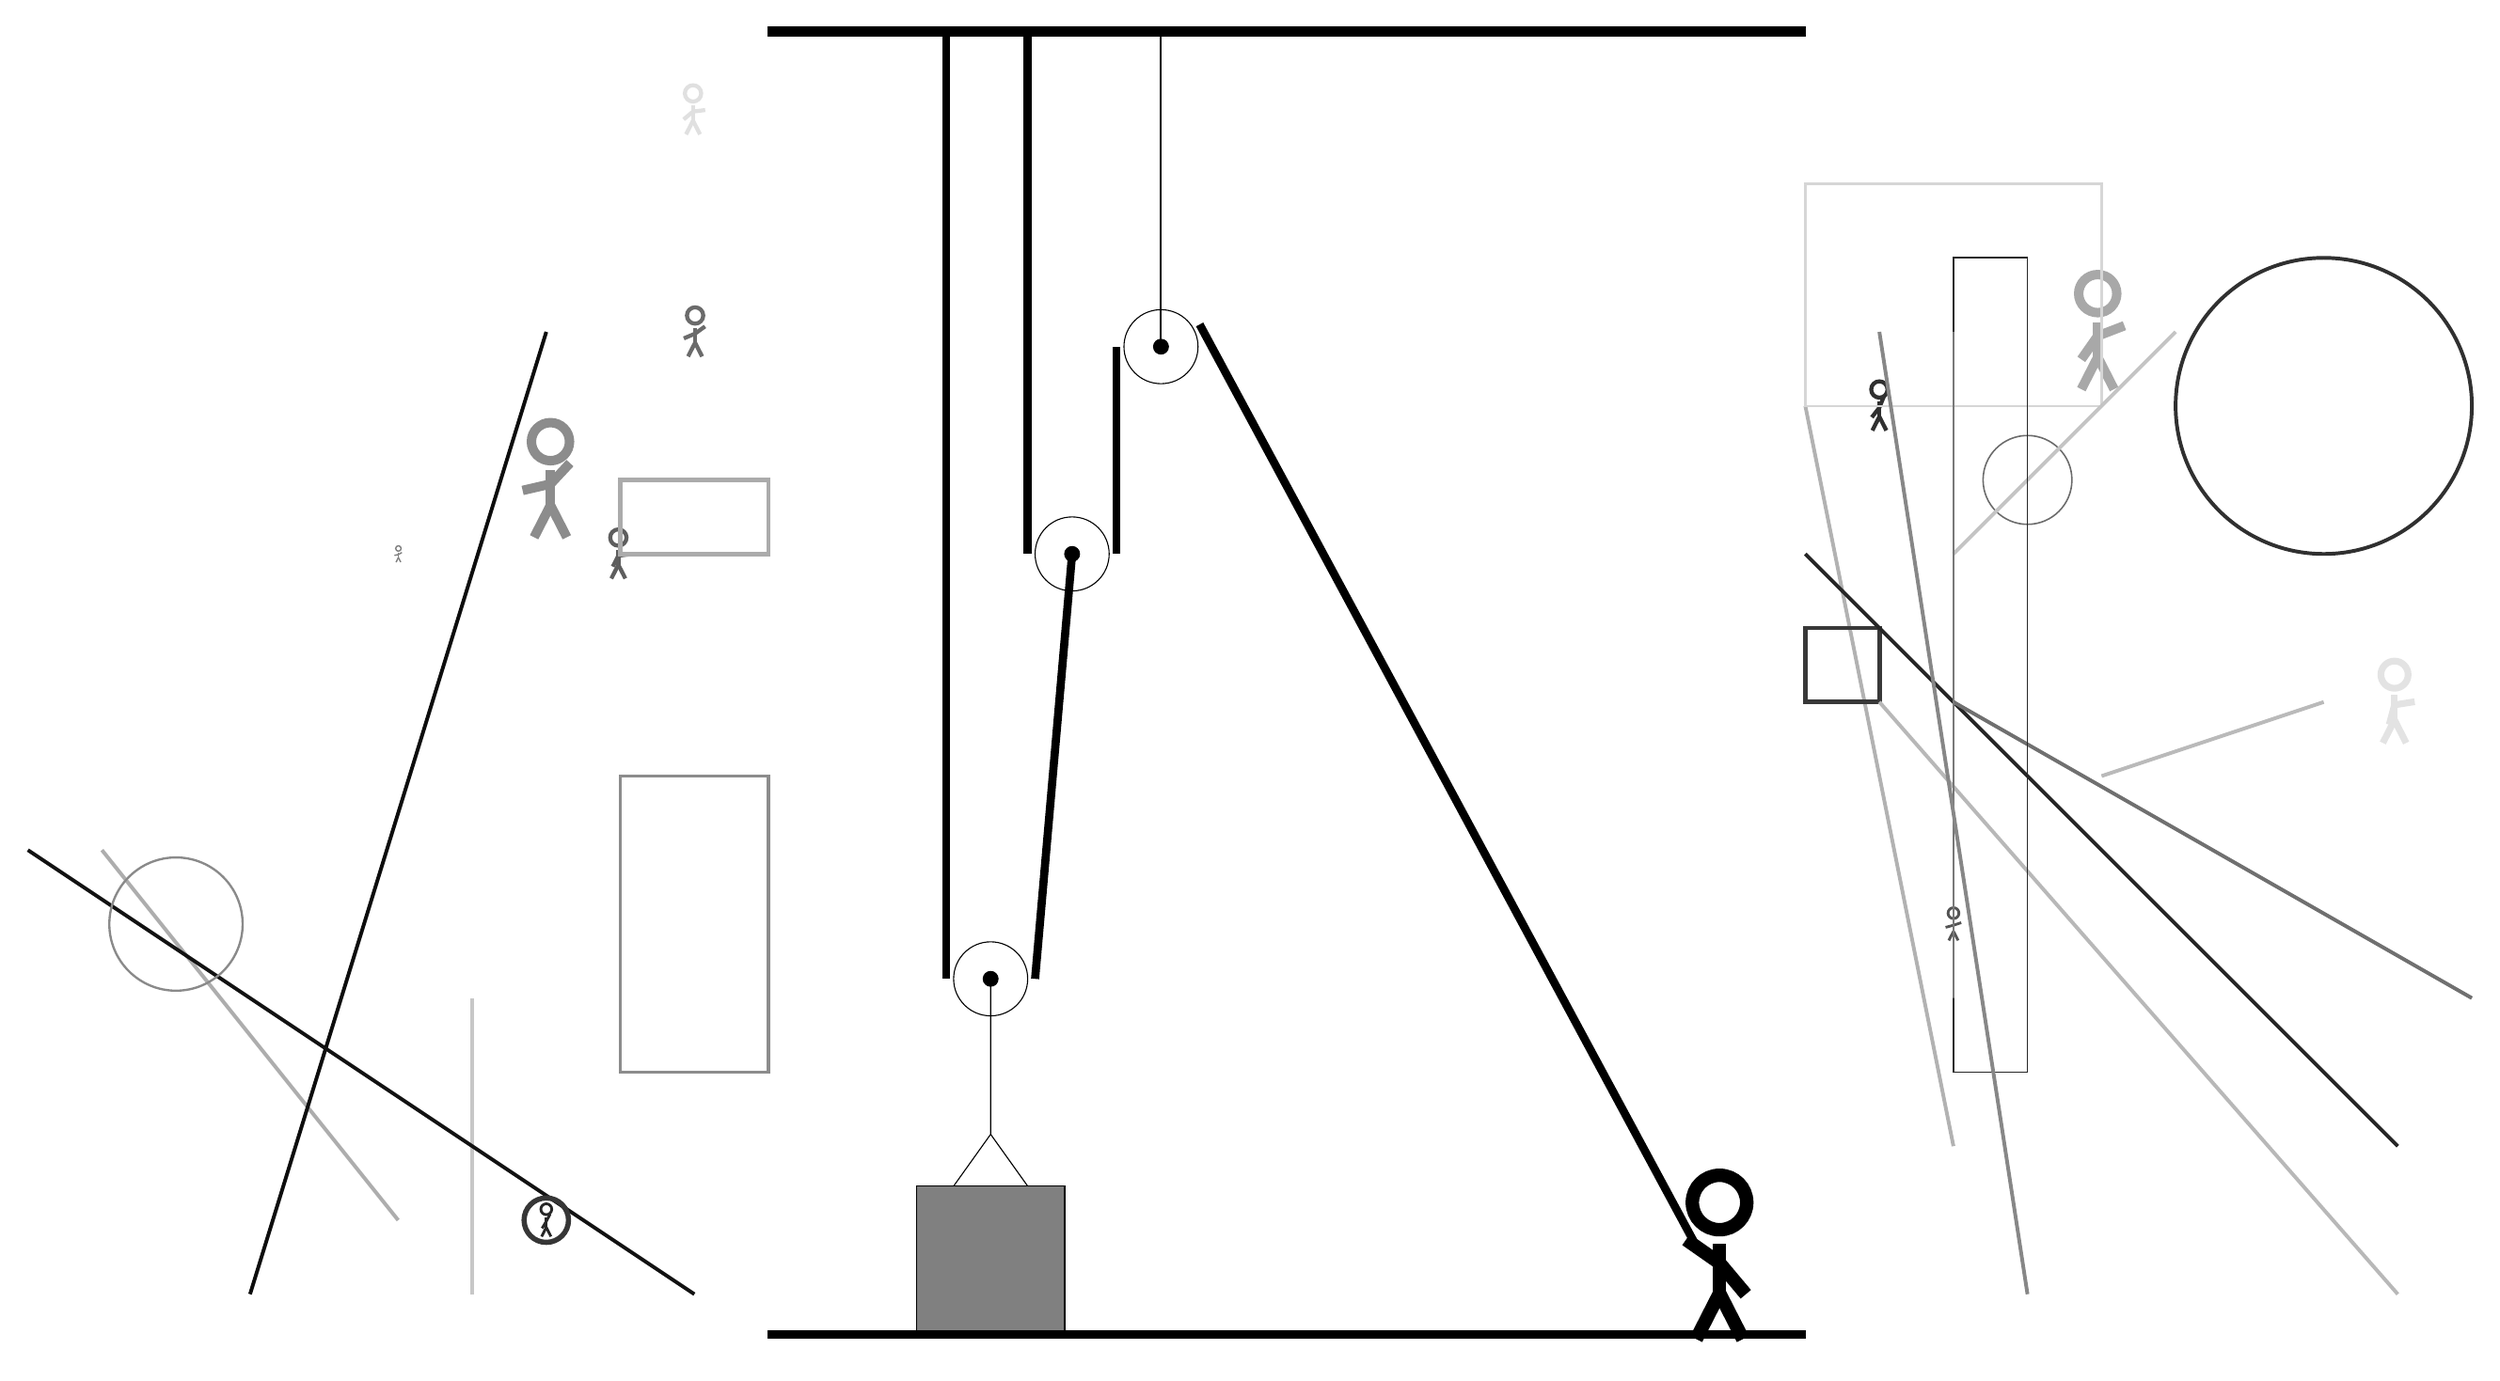
\begin{tikzpicture}
			%%%%% START %%%%%
			
			\draw[fill=black] (-2, 14) rectangle (12, 14.125);
			
			\draw (1, 1.26) circle (0.5);
			\draw[fill=black] (1, 1.26) circle (0.1);
			
			\draw (2.1, 7.0) circle (0.5);
			\draw[fill=black] (2.1, 7.0) circle (0.1);
			
			\draw (3.3, 9.8) circle (0.5);
			\draw[fill=black] (3.3, 9.8) circle (0.1);
			\draw[thick] (3.3, 9.8) -- (3.3, 14);
			
			\draw (1, 1.26) -- (1, -0.84) -- (0.5, -1.54) -- (1.5, -1.54) -- (1, -0.84);
			\draw[fill=black!50] (0, -1.54) rectangle (2, -3.54);
			
			\draw[line width=1.1mm] (0.4, 14) -- (0.4, 1.26);
			\centerarc[line width=1.1mm](1, 1.26)(180:360:0.6);
			\draw[line width=1.1mm](1.6, 1.26) -- (2.1, 7.0);
			\draw[line width=1.1mm] (1.5, 14) -- (1.5, 7.0);
			\centerarc[line width=1.1mm](2.1, 7.0)(180:360:0.6);
			\draw[line width=1.1mm](2.7, 7.0) -- (2.7, 9.8);
			\centerarc[line width=1.1mm](3.3, 9.8)(30:180:0.6);
			\draw[line width=1.1mm] (3.822, 10.1) -- (10.5, -2.3);
			
			\node at (10.8, -2.5) {\Strichmaxerl[10][-35][-50]};
			
			\node[line width=0.4mm, color=black!45] at (-5, 8) {\Strichmaxerl[7][13][47]};
			
			\draw[line width=0.5mm, color=black!32](-7, -2) -- (-11, 3);
			\draw [line width=0.2mm, color=black!98](17, 3) circle (0.0);
			\node[line width=0.6mm, color=black!81] at (13, 9) {\Strichmaxerl[3][52][68]};
			\node[line width=0.5mm, color=black!11] at (20, 5) {\Strichmaxerl[5][75][9]};
			
			\draw[line width=0.5mm, color=black!95](-5, 10) -- (-9, -3);
			
			\draw[line width=0.5mm, color=black!30](12, 9) -- (14, -1);
			\draw[line width=0.6mm, color=black!78] (13, 5) rectangle (12, 6);
			\draw[line width=0.5mm, color=black!22](-6, -3) -- (-6, 1);
			
			\node[line width=0.6mm, color=black!12] at (-3, 13) {\Strichmaxerl[3][40][7]};
			\node[line width=0.5mm, color=black!34] at (16, 10) {\Strichmaxerl[7][55][21]};
			
			\node[line width=0.7mm, color=black!63] at (-4, 7) {\Strichmaxerl[3][63][7]};
			\draw[line width=0.5mm, color=black!85](12, 7) -- (20, -1);
			
			\node[line width=0.4mm, color=black!50] at (-7, 7) {\Strichmaxerl[1][12][30]};
			\draw[line width=0.5mm, color=black!56](14, 5) -- (21, 1);
			\node[line width=0.6mm, color=black!67] at (14, 2) {\Strichmaxerl[2][15][18]};
			
			\draw [line width=0.2mm, color=black!58](15, 8) circle (0.6);
			\draw[line width=0.5mm, color=black!28](13, 5) -- (20, -3);
			\draw[line width=0.4mm, color=black!45] (-4, 4) rectangle (-2, 0);
			\draw[line width=0.5mm, color=black!93](-3, -3) -- (-12, 3);
			\node[line width=0.2mm, color=black!58] at (-3, 10) {\Strichmaxerl[3][23][36]};
			
			\node[line width=0.7mm, color=black!85] at (-5, -2) {\Strichmaxerl[2][59][62]};
			\draw[line width=0.3mm, color=black!16] (12, 12) rectangle (16, 9);
			\draw [line width=0.5mm, color=black!81](19, 9) circle (2.0);
			\draw[line width=0.6mm, color=black!33] (-2, 7) rectangle (-4, 8);
			
			\draw[line width=0.5mm, color=black!23](17, 10) -- (14, 7);
			
			\draw[line width=0.2mm, color=black!85] (14, 11) rectangle (15, 0);
			\draw [line width=0.3mm, color=black!46](-10, 2) circle (0.9);
			\draw [line width=0.7mm, color=black!79](-5, -2) circle (0.3);
			
			\draw[line width=0.2mm, color=black!53] (14, 1) rectangle (14, 10);
			\draw[line width=0.5mm, color=black!47](13, 10) -- (15, -3);
			\draw[line width=0.5mm, color=black!27](16, 4) -- (19, 5);
			
			\draw[fill=black] (-2, -3.5) rectangle (12, -3.6);
			
			%%%%% END %%%%%
		\end{tikzpicture}
	\end{figure}	
\end{document}